\chapter{Current progress}
Recent developments in quantum dot based qubits have managed to convince us that good quality qubits are just around the corner. \cite{petta} have managed to synthesize Si double quantum dot based qubits which have strong coupling between the single electron in the dot to the photonic field of a microwave cavity. This allows for entanglement and coupling over large distances. This enables us to envision devices which are quantum coupled or entangled with each other even if far away from each other. 
\par
Anyway coming back to the point, their set up is a double quantum dot qubit placed in a microwave cavity. This is quite similar to our setup in which we have two qubits place in a cavity.\\ 
\begin{figure}
\centering
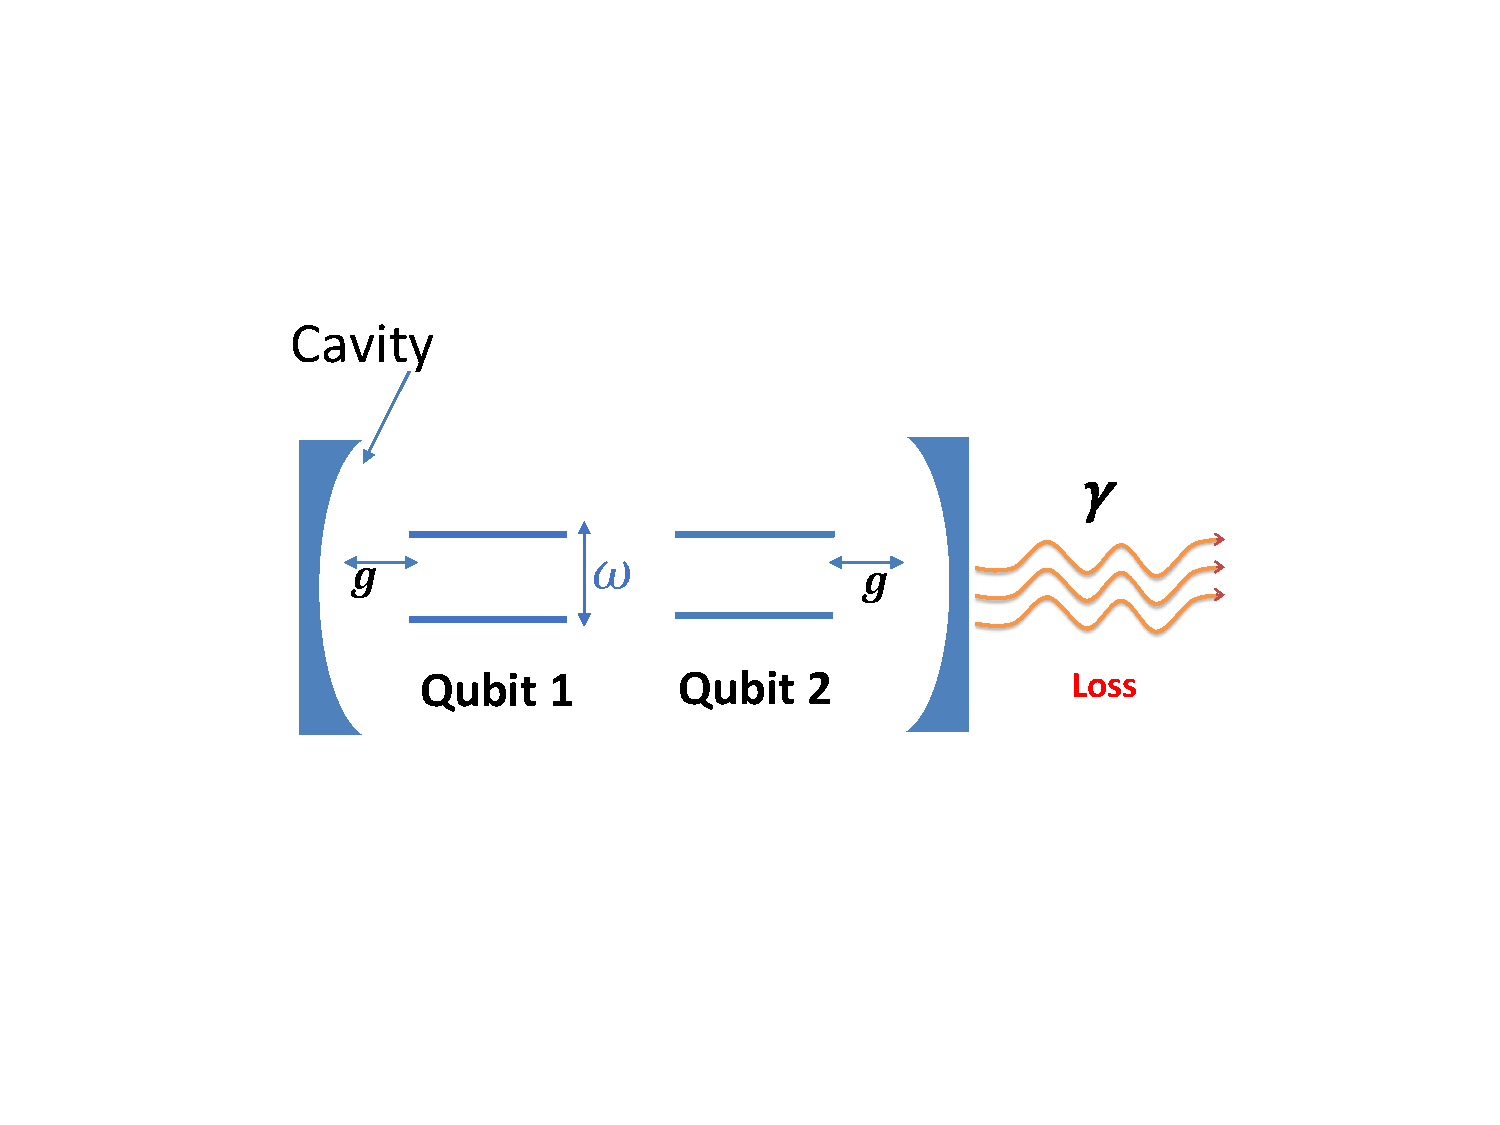
\includegraphics[width=0.8\textwidth]{Figr1a} 
\end{figure}
\par
The range of $\omega_{c}$ is about the range of $\omega_{q}$.  As we saw last time it is better to vary the field $g(t)$. Only if it is specific range and not otherwise looking for answers we hit upon \cite{hot_gates}. By performing certain algebraic manipulations they manage to decouple the qubits from the cavity at specific intervals of time. The only way the qubits interact is via the cavity. If one moves the cavity there wont be any path by which they could decohere.This brings about long coherence times, and allows on to operate at "elevated temperatures" 1K to 4K. These temperatures are far higher than what one usually encounters in this field eg.mK. It also would allow us to make classical connections to quantum hardware.Here their system is exactly the same as ours but they require that the qubit level spacing $\omega_{q}$ is less than of $\omega_{c}$. This puts it out of the range of \cite{petta}.
\par
Basically we need a way in which one could efficiently develop control field temporal variation to implement a specific gate.  It must be like an algorithm where on performing a series of steps either repeatedly or otherwise one ends up with a control field that performs the unitary we want. This it must be able to do to a tolerable (practical) level of error. Few of the algorithms that do this are:
\begin{itemize}
    \item Krotov as in \cite{tannor1992control}
    \item \cite{zhu1998rapid}
    \item GRAPE  \cite{khaneja2005optimal}
    \item CRAB (Chopped RAndom Basis) \cite{doria}, \cite{caneva2011chopped}
    \item DCRAB (Dressed Chopped RAndom Basis) \cite{rach2015dressing}
    \item GOAT (Gradient Optimization of Analytic conTrols) \cite{machnes2015gradient}
\end{itemize}
\par
Krotov \citep{tannor1992control} and \citep{zhu1998rapid} were combined together in a single algorithm by \citep{maday2003new}.   GRAPE \citep{khaneja2005optimal} is Gradient Ascent by Pulse Engineering. It explicitly makes use of derivatives. When unable to do so it calculates a suitable thing which emulates them. Primarily they are gradient descent algorithms. They always get a solution but sometimes require appalling amount of computational resources. CRAB and its improvements DCRAB \citep{rach2015dressing} are basically non gradient methods which make use of analytic functions. These methods have may fail to reach the optimal solution but do so quickly on being successful.
\par
GOAT  \citep{machnes2015gradient} combines the best features of all before it to achieve high accuracy without compromising on speed. It is some what more complicated though.
\par
To keep things simple lets start with Krotov by \citep{tannor1992control} algorithm in the form given by  \citep{maday2003new}. To gain deeper understanding, first we must generalize our system. So instead of   

   





\section{Introduction}
 Say, we want to apply a target unitary $T_{s} $ on our quantum system. Let the Hamiltonian of our system be $\mathcal{H} $. The Lindbladian operators associated with it be $\{ L_{m} \}$. The Hamiltonian of the system is given by 
\begin{align}\label{Hamiltonian form}
    H &= H_{0} + g(t) H_{I} 
\end{align}

where,
\begin{enumerate}
    \item[$H_{0} :$] bare Hamiltonian
    \item[$ g(t) :$] control field as a function of time.
    \item[$ H _{ I} :$] control Hamiltonian (interaction Hamiltonian)
\end{enumerate}

The system is assumed to be governed by Lindblad equation.
\begin{align}
    \dot{\rho} = - i\comm{H}{\rho} + \mathcal{L}(\rho)
\end{align}

where,
\[
 \mathcal{L}(\rho) = \gamma\sum_{k} L_{m} \rho L_{m}^{\dagger} - 0.5 \anticommutator{L_{m}^{\dagger}L_{m}}{ \rho}
\]

The application of a target unitary $T_{s} $ on the system can be translated in mathematical terms (in open quantum systems formalism) as follows :
\[
 \rho \rightarrow T_{s}  \rho T_{s} ^{\dagger}
\]
%https://www.overleaf.com/1524532912qjmbpfcwcpbv
So, the question at hand is what must be the form of $ g (t)$
 such that for any $\rho $ if we let the system evolve (under the influence of the  control field  $g (t) $ ) we get the final state $T_{s} \rho  T_{s} ^{\dagger}$.

\section{Taking advice from other sources}
%Some advice from \cite{2018EPJST.227..203S}
\cite{2018EPJST.227..203S} have  discussed a similar problem with one major difference. Instead of implementing a specific unitary gate they have a fixed initial state which they wish to evolve to a fixed target state.  They wish to find know how would $ g(t)$ have to vary for the quantum system to evolve as close as possible to the target state. They discuss how this has already been done in many ways for closed quantum systems. The one which they focus upon is given in \cite{2012JChPh.136j4103R}.


Let us have quick review of it. Assuming we have a closed quantum system which we want to drive from a fixed state $ \ket{\psi _{0}}$ to a target state $ \ket{\tau} $. The Hamiltonian of the system is as in \eqref{Hamiltonian form}.
For this the write down a cost function $J$ as follows (details are in  \cite{2018EPJST.227..203S}) :
\begin{align}\label{cost_function}
    J[\ket{\psi}, \ket{\chi}, g(t)] &= \expval{Q}{\psi(T)} - 2Re\int_{0}^{T}dt \matrixelement{\chi(t)}{\dv{}{t} +  iH(t)}{\psi(t)}  - \alpha \int_{0}^{T}dt g^{2}(t)
\end{align}
where $ Q = \dyad{\tau}$. The first order variation $δJ$ is set to zero to obtain a set of equations, namely
\begin{align}\label{anal-krotov}
    i\ket{\dot{\psi}(t)} &=  H(t)\ket{\psi(t)},\text{with} \ket{\psi(0)} = \ket{\psi_{0}}\\
    i\ket{\dot{\chi}(t)} &= H(t)\ket{\chi(t)},\text{with} \ket{\chi(T)} = Q\ket{\psi(T)}\\
    g(t) &= \frac{-1}{\alpha}\text{Im}\matrixelement{\chi(t)}{\mu}{\psi(t)}
\end{align}


Following \cite{2012JChPh.136j4103R},   Eqns. \eqref{anal-krotov} could be solved self-consistently  as below,
\begin{align}\label{ansatz_krotov}
    i\ket{\dot{\psi}^{(k)}(t)} &=  H^{(k)}(t) \ket{\psi^{(k)}(t)},\text{with} \ket{\psi^{(k)}(0)} = \ket{\psi_{0}}\\
    i\ket{\dot{\chi}^{(k)}(t)} &= H^{(k)}(t) \ket{\chi^{(k)}(t)},\text{with} \ket{\chi^{(k)}(T)} = Q\ket{\psi^{(k)}(T)}\\
    g^{(k)}(t) &= (1 - \delta)\tilde{g}^{(k-1)}(t) -  \dfrac{\delta}{\alpha}\text{Im}\matrixelement{\chi^{(k-1)}(t)}{\mu}{\psi^{(k)}(t)}\\
    g^{(k)}(t) &= (1 - \eta)\tilde{g}^{(k)}(t) -  \dfrac{\delta}{\alpha}\text{Im}\matrixelement{\chi^{(k)}(t)}{\mu}{\psi^{(k)}(t)}
\end{align}

For open quantum systems \cite{2018EPJST.227..203S} suggest to move from the Hilbert space to Liouville space, which involves vectorizing the density matrix $\rho$ as $\ket{\psi}\rangle$. So the problem goes from 
 \begin{align}\label{Hilbert_liou:1}
     \rho_{0} &\rightarrow \rho_{f}\\
     \dot{\rho} &= - i\comm{H}{\rho} + \gamma\sum_{k} \left(L_{m} \rho L_{m}^{\dagger} - 0.5 \anticommutator{L_{m}^{\dagger}L_{m}}{ \rho}\right)\\
\text{to, }   
    \ket{\psi_{0}}\rangle &\rightarrow \ket{\tau}\rangle\\
    i\ket{\dot{\psi}(t)}\rangle &= A(t)\ket{\psi(t)}\rangle,  \text{ where}\\
    A(t) &= I\otimes H(t) - H^{*}(t)\otimes I + i\gamma\sum_{k} \left(
    L_{m}^{T}\otimes L_{m} - 0.5\left( I \otimes L_{m}^{\dagger} L_{m} + L_{m}^{T} L_{m}^{*} \otimes I\right)\right)
\end{align}
\section{Back to our problem}
Coming to our problem we have,
\begin{align}\label{Hilbert:2}
    \rho &\rightarrow T_{s}\rho T_{s}\\
    \dot{\rho} &= - i\comm{H}{\rho} + \gamma
    \sum_{k} \left(L_{m} \rho L_{m}^{\dagger} - 0.5\anticommutator{L_{m}^{\dagger}L_{m}}{ \rho}\right)
\end{align}
Moving to Liouville space one can rewrite it as, 
 \begin{align}\label{Liouville:2}
     \ket{\psi}\rangle &\rightarrow T_{s}^{T} \otimes T_{s}\ket{\psi}\rangle\\
     i\ket{\dot{\psi}(t)}\rangle &= A(t)\ket{\psi(t)}\rangle
 \end{align}
where $A(t)$ is as given before in equation \eqref{Hilbert_liou:1}. From now on wards, let $T_{s}^{T} \otimes T_{s}$ be called as $T$.  But unlike \cite{2018EPJST.227..203S} instead of initial and final states we have the target unitary $T$. So, we cannot write the  same cost function and optimize it to get the desired control field. 
\section{Putting it all together}
Since,
\begin{align}
    i\ket{\dot{\psi}(t)}\rangle &= A(t)\ket{\psi(t)}\rangle\\
    \ket{\psi(t)}\rangle &= e^{-i\int_{0}^{T}dt A(t)}\ket{\psi(0)}
\end{align}
Let $e^{-i\int_{0}^{T}dt A(t)}$ be denoted by $\mathcal{L}$. One can approximate it as follows:
\begin{align}
    \mathcal{L}&=e^{-i\int_{0}^{T}dt A(t)}\\
    \mathcal{L}&= \prod_{k = N}^{1} \mathcal{L}_{k}\\
\end{align}
% $\mathcal{L}&=e^{-i\sum_{0}^{T}\delta t A(t)} = \prod_{k = N}^{1}$
where $\mathcal{L}_{k} = e^{-iA(t_{k})\delta t}$.
Let us define a few other terms.
\begin{align}\label{some_def}
    \mathcal{L}^{d}_{k} &= \mathcal{L}_{N}\mathcal{L}_{N-1}\ldots X_{k} \mathcal{L}_{k}\ldots \mathcal{L}_{2}\mathcal{L}_{1}\\
    X_{k} &= I\otimes H_{I}(t) - H_{I}^{*}(t)\otimes I 
\end{align}
%\phi &=  
%    J[g] &= -\phi^{*} \phi\\
Now we shall define $F[g] = - Tr((T - \mathcal{L})^{\dagger}(T - \mathcal{L}))$ to be our fidelity measure as in \cite{khaneja2005optimal}. Next we need to devise an update step for the control field which would improve the fidelity. Following \cite{khaneja2005optimal} we have 
\begin{align}\label{update_step}
    g(t_{k+1})&= g(t_{k}) + \pdv{F}{g(t_{k})} \text{, or}\\
    g_{k+1} &=    g_{k}   + \epsilon\pdv{F}{g_{k}}
\end{align}
$\epsilon$ is  constant which would depend on the speed at which one would want to converge,etc.
\begin{align}
    \pdv{F}{g_{k}}&=Tr((T - \pdv{\mathcal{L}}{g_{k}})^{\dagger}(T - \mathcal{L})) + Tr((T - \mathcal{L})^{\dagger}(T - \pdv{\mathcal{L}}{g_{k}})) \\
    \pdv{F}{g_{k}}&=  Tr((T - \mathcal{L}^{d}_{k})^{\dagger}(T - \mathcal{L})) + Tr((T - \mathcal{L})^{\dagger}(T - \mathcal{L}^{d}_{k})))\\
    \mathcal{L}^{d}_{k}=\pdv{\mathcal{L}}{g_{k}} &= \pdv{(\mathcal{L}_{N}\mathcal{L}_{N-1}\ldots  \mathcal{L}_{k}\ldots \mathcal{L}_{2}\mathcal{L}_{1})}{g_{k}}\\
    \mathcal{L}^{d}_{k}=\pdv{\mathcal{L}}{g_{k}} &= \mathcal{L}_{N}\mathcal{L}_{N-1}\ldots \pdv{ \mathcal{L}_{k}}{g_{k}}\ldots \mathcal{L}_{2}\mathcal{L}_{1}\\
    \mathcal{L}^{d}_{k} &= \mathcal{L}_{N}\mathcal{L}_{N-1}\ldots X_{k} \mathcal{L}_{k}\ldots \mathcal{L}_{2}\mathcal{L}_{1}\\
    X_{k} &= I\otimes H_{I}(t) - H_{I}^{*}(t)\otimes I 
\end{align}
%$X_{k}$
\subsection{Steps to find optimal control field }
%$g_{opt}(t)$
\begin{enumerate}
    \item Start with a random $g_{rand}(t)$.
    \item Calculate fidelity $F$.
    \item Update $g(t) $ using  \Eqref{update_step}
    \item If fidelity $F$ calculated from new $g(t) $ differs from old one by more than $\mu$, then go to step 3.
    \item Terminate.
\end{enumerate}



